\section{System Overview}
\label{sec:overview}

The OLCF deployed Spider 1 file system in 2008~\cite{spider1}. It served as a
center-wide file system for all OLCF resources, including Jaguar~\cite{jaguar}
for 5 years, and was decommissioned in 2013. Our analysis of Spider 1 I/O
workload was presented in~\cite{spider1-workload}. 

The OLCF deployed Spider 2 file system in 2012~\cite{spider2}. Spider 2 is also
a center-wide shared resource and serves all current OLCF platforms, including the Titan supercomputer~\cite{titan}.

Both Spider 1 and 2 were architected, deployed, and operated by the OLCF staff.
Both file systems use the Lustre technology~\cite{Lustre}.

Similar to the Spider 1 file system, Spider 2 also uses Data Direct Networks'
(DDN) block-level RAID controllers. In Spider 2 these controllers are connected
to external nodes via Infiniband FDR technology. These external nodes serve as
Lustre I/O servers.

There are 72 DDN  SFA12KX RAID controllers in Spider 2. Each controller runs as
a tandem pair with another for redundancy. Each pair is called a ``couplet.''
Each couplet is connected to ten disk enclosures hosting 560 2 TB near-line SAS
disks. These 560 disks are organized in 8+2 RAID 6 arrays. Therefore, each
couplet controls 56 RAID sets. Each couplet is also connected to 8 external
servers and each server are primarily assigned to control and operate 7 of
these RAID sets. Fail-over pairs between external servers are defined for
redundancy.

Each external server acts as a Lustre Object Storage Server (OSS) and builds a
Lustre Object Storage Target (OST) on one of these exported RAID sets. There
are 288 total Lustre OSSes, and 2,106 Lustre OSTs in Spider 2.

These resources are organized in two separate name spaces in Spider 2. These
namespaces are identified as ``atlas 1'' and ``atlas 2.'' Namespaces are built
on non-overlapping Spider 2 hardware resources. Figure~\ref{fig:arch} shows the conceptual Spider 2 architecture. 

Spider 2 storage system was rated and tested for 1.4 TB/s aggregate read and
1.2 TB/s write performance. At the Lustre file system level these translate
into +1 TB/s aggregate read and write performance.

Table~\ref{table:spider12} highlights key characteristics of the Spider 1 and 2 file systems.

The OLCF also built a comprehensive monitoring system for operating the Spider
2 resources, as well as other OLCF systems. More details on these can be found
in~\cite{olcf-monitoring}. Some of these monitoring tools have been in-house
developed at the OLCF. For monitoring the DDN systems, OLCF staff has been
using a tool called ``DDNTool.'' The DDNTool has been coded for Spider 1
originally and later updated for Spider 2.  


\begin{figure}[!t]
\centering
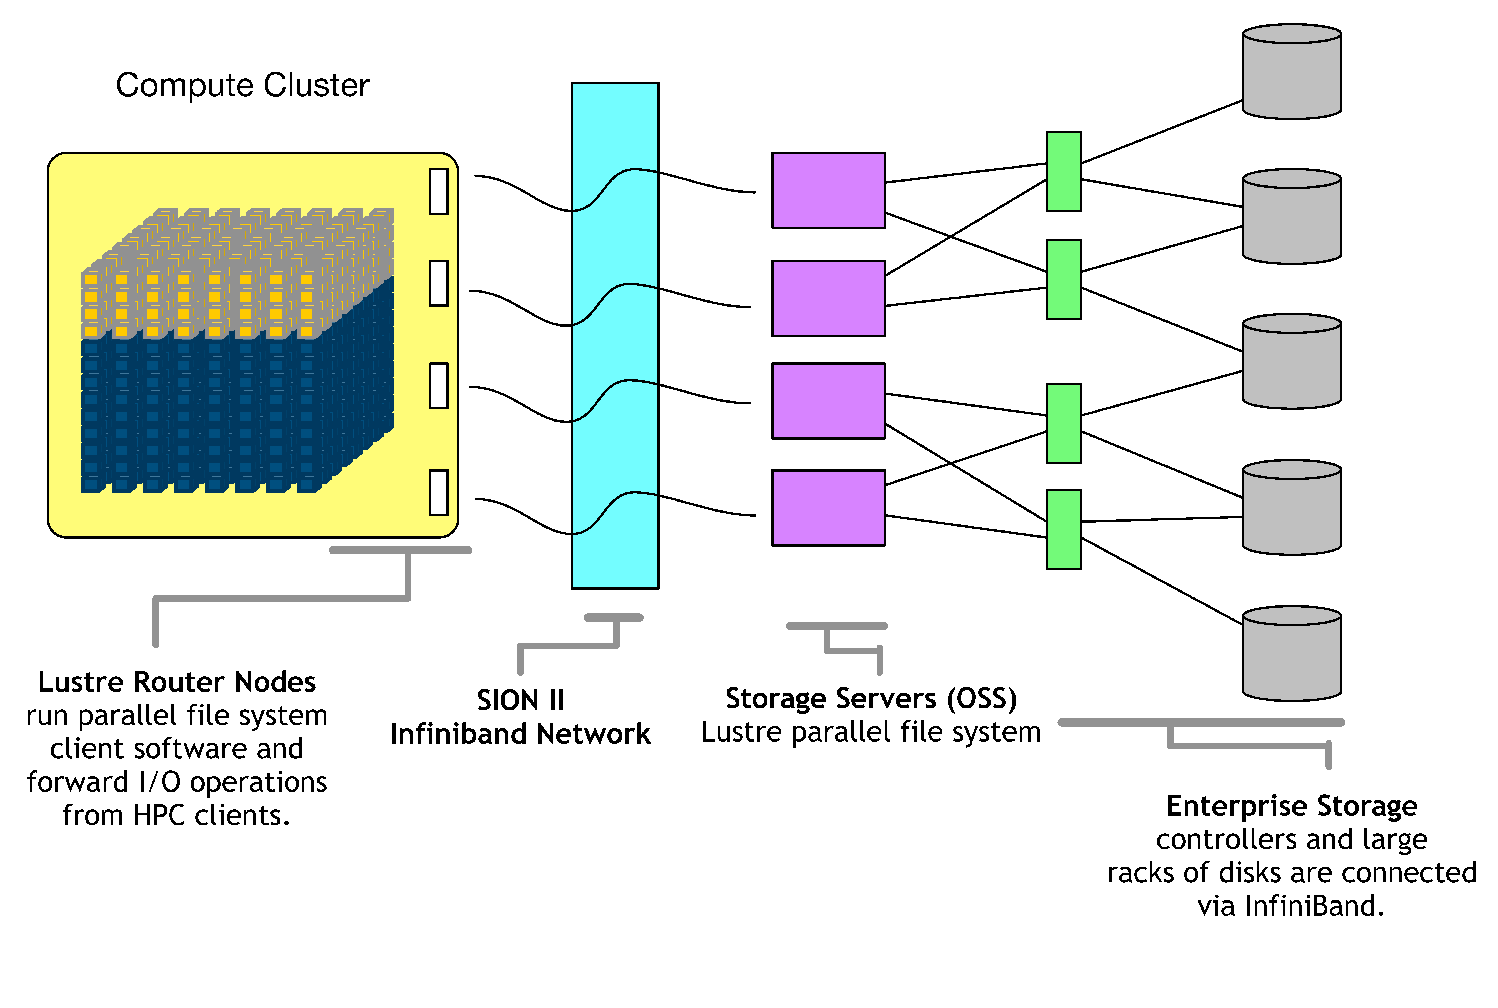
\includegraphics[width=0.45\textwidth]{./figs/spider2arch.ps}
\vspace{-0.1in}
\centering
\caption{Spider Architecture}
\label{fig:arch}
\end{figure}

\begin{table}{h!}
\begin{center}
\begin{tabular}{l||l|l}
 Spec & Spider 1 & Spider 2\\
\hline
Bandwidth & 240 GB/s & 1 TB/s \\
\
Capacity & 10 PB & 32 PB \\
Addmore \\
\end{tabular}
\end{center}
\label{table:spider12}
\end{table}


\subsection{Monitoring tool}
DDNTool \cite{ddntool10:ross} was developed to monitor the DDN S2A and SFA storage system RAID controllers. Since the two DDN architectures have very different monitoring API's, there are actually two completely separate programs:  DDNTool for the S2A architecture and DDNTool\_v2 for the SFA architecture.  The two tools are very different in their implementations - DDNTool is a C++ program that communicates with the disk controllers directly over TCP/IP while DDNTool\_v2 is a Python program that interfaces with a vendor-supplied python library which handles the low level communication - but they both accomplish the same basic task.  The tools poll each controller for various pieces of information (e.g. I/O request sizes, write and read bandwidths) at regular rates and store this information in a MySQL database.  The database is not actually used for long term storage.  In fact, at each poll interval, the old data is overwritten with new data.  By storing a the data in a database, though, the data is available to numerous clients via a well-documented API.  This allows multiple users to search and query in real-time.

